\documentclass[10pt,notitlepage,openany]{scrbook}
\usepackage{anysize}
\paperwidth = 13.95cm
\paperheight = 21.6cm
\marginsize{1.5cm}{1.5cm}{1.5cm}{1.5cm} %\marginsize{izq}{der}{sup}{inf }

\usepackage{bera}		% Define el tipo de letra
\usepackage{arev}
\usepackage{hyperref}

%\oddsidemargin = 4cm
%\evensidemargin = 2cm
%\usepackage[left=6.8cm,top=6cm,right=0cm]{geometry} 
%left 0=2.8,
%\documentclass[bsc,draft,singlespacing]{csthesis}
%\documentclass[bsc,doublespacing]{csthesis}
      
\usepackage[spanish]{babel}     % Idioma de Captulos y dems
\usepackage[T1]{fontenc} 
\usepackage[utf8x]{inputenc}


\usepackage{titlesec}
\titleformat{\chapter}[hang]{\LARGE\bfseries}{\thechapter}{1em}{\bfseries}
\titlespacing{\chapter}{0pt}{-1cm}{1cm}


\usepackage{hyperref}



\usepackage{mathcomp}
\usepackage{latexsym}
\usepackage{pifont}
\usepackage{amsfonts}
\usepackage{amssymb}
\usepackage{wasysym}
\usepackage{colortbl}
\usepackage{multicol} 
\usepackage{booktabs}


\usepackage{graphicx}


\setlength{\parindent}{0cm}
\setlength{\parskip}{0.3cm}


\title{Manual Reloj MA 32-2}
\author{Galeras Digital}

\begin{document}
\pagestyle{empty}

\begin{figure}[ht]
	\begin{center}
		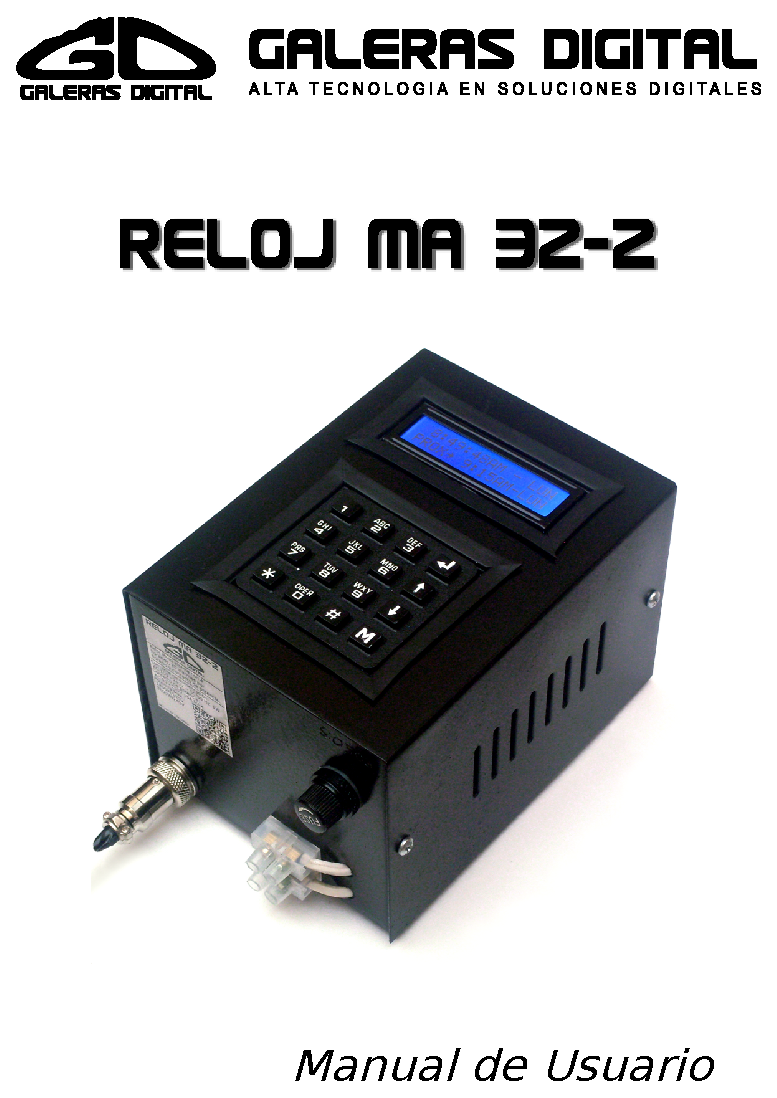
\includegraphics[width=1\textwidth]{./figuras/tapam.eps} 
	\end{center}
\end{figure}


\tableofcontents 
\pagestyle{plain}
\chapter{Descripción General}

El Reloj MA 32-2 es un dispositivo electrónico digital que cuenta con un reloj calendario y la posibilidad de programar 30 distintas alarmas con diversas opciones de timbrado en cuatro diferentes tipos de horarios. Maneja un contacto de potencia capaz de soportar hasta 15A a 120VAC (1800W), una memoria interna tipo EEPROM donde se almacena la configuración de las alarmas sin perder los datos por hasta 40 años, una pila tipo CR2032 para no perder la fecha y hora en caso de fallas del fluido eléctrico y un menú en pantalla LCD que facilita su manejo.

\textit{Ventajas:}

La precisión en el timbre para el cambio de hora, es de gran importancia para toda la comunidad educativa, pero especialmente para el docente quien podrá programar sus actividades de clase con la plena seguridad de que el timbre de cambio de hora sonará con una precisión de segundos. 

La labor diaria y constante del toque del timbre se olvidará por completo, ya que el Reloj MA 32-2 se programa por una sola vez y no requiere de ninguna otra operación.

\section{Características}

\textit{Cuatro Horarios:} El Reloj MA 32-2 permite programar cuatro horarios distintos, cada uno hasta con 30 timbrasos, los cuales se pueden asignar independientemente a los diferentes días de la semana.

\textit{Fácil Manejo:} Su programación es muy sencilla y se realiza por una sola vez, esta no se borrará aunque se suspenda el fluido eléctrico.

\textit{Pila de respaldo:} El Reloj MA 32-2 cuenta con una pila de respaldo la cual permite al sistema mantener la fecha y la hora en caso de cortes en el fluido eléctricºo. La pila usada, CR2032 tiene una duración aproximada de 10 años y se consigue fácilmente en cualquier relojería o tienda electronica.

\textit{Pantalla LCD:} Su pantalla LCD retro iluminada, facilita la programación y muestra constantemente la hora exacta y la hora del próximo timbre. 

\textit{Teclado Numérico:} Su teclado numérico y de funciones permite una fácil programación de los timbrados y el cambio de horario.

\textit{Adaptabilidad:} El Reloj MA 32-2 se instala y adapta fácilmente a cualquier sistema de timbre, chicharra o sistema de alarma.

\textit{Seguridad:} El Reloj MA 32-2 posee un sistema de seguridad que solicita una clave o contraseña, para evitar que personas no autorizadas accedan o modifiquen la programación.

\textit{Calidad:} El Reloj MA 32-2 está elaborado con materiales de altísima calidad lo que garantiza un funcionamiento preciso e ininterrumpido durante muchos años.


\newpage

\section{Vista frontal}

En la parte frontal se encuentra una pantalla LCD y un teclado de números y funciones con los cuales se opera el Reloj MA 32-2.

\begin{figure}[ht] 
        \caption[Vista frontal]{Vista frontal}
        \begin{center}
                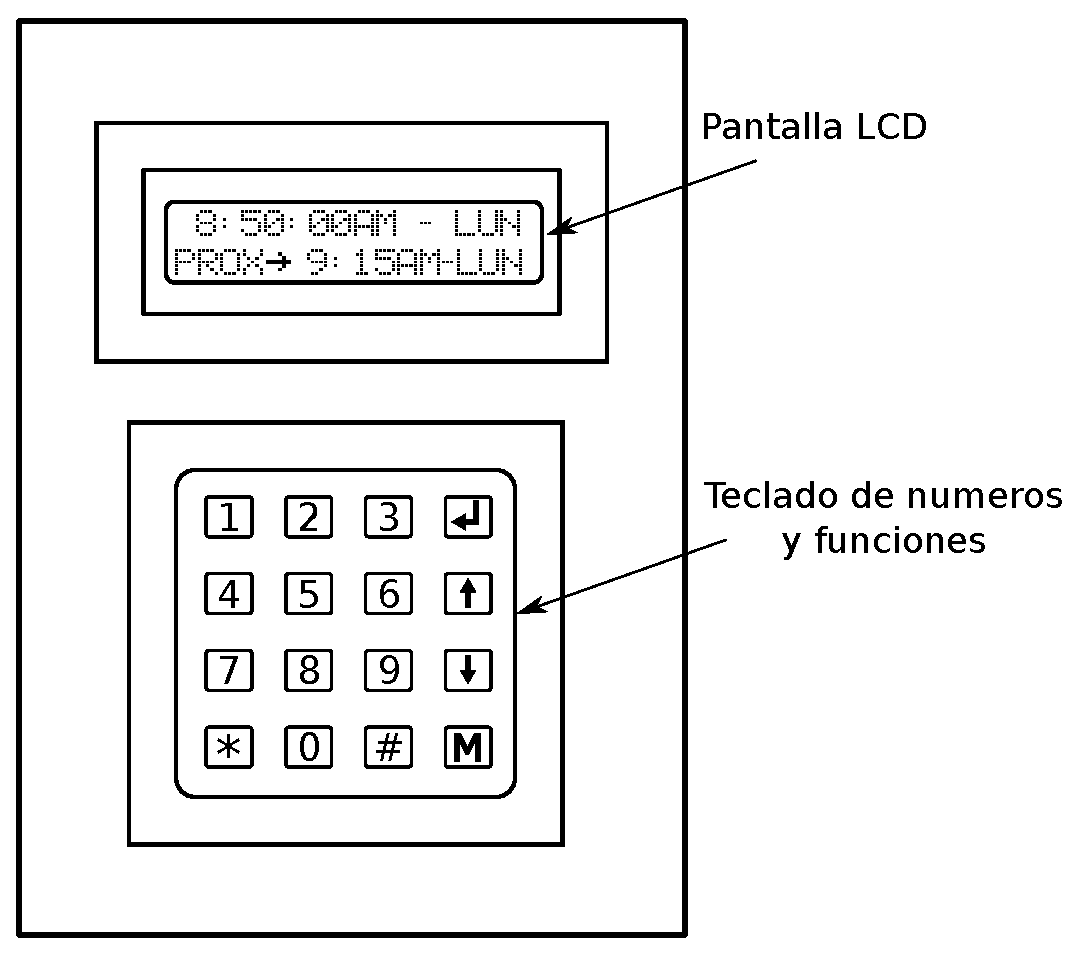
\includegraphics[width=0.75\textwidth]{./figuras/frente1.eps} 
        \end{center}
	\label{frente1}
\end{figure}

\newpage

\section{Vista inferior}

En la parte inferior se encuentra la entrada de corriente de 12VDC, un fusible de 15A que protege el contacto interno y el conector de potencia donde se conecta el circuito de los timbres.

\begin{figure}[ht]
        \caption[Vista inferior]{Vista inferior}
        \begin{center}
                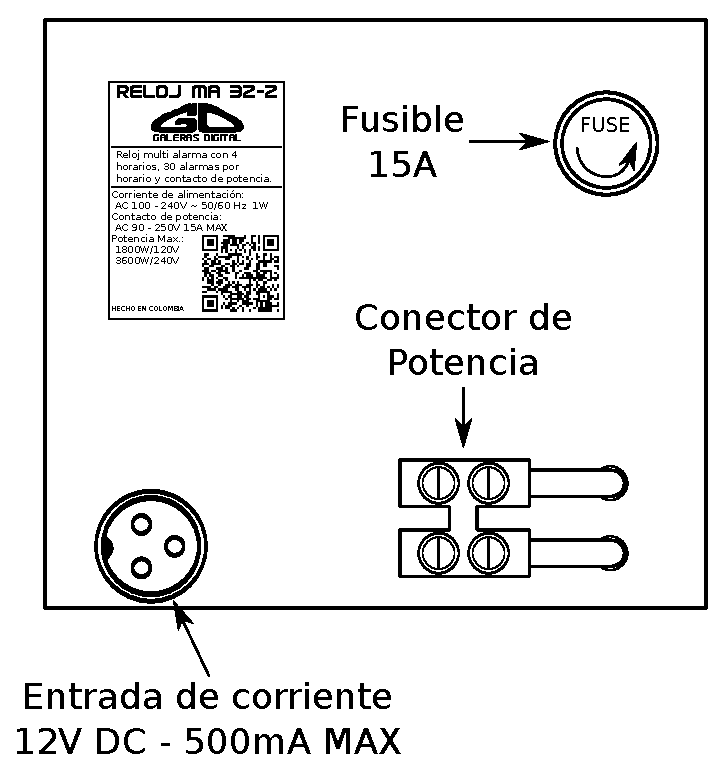
\includegraphics[width=0.6\textwidth]{./figuras/inferior1.eps} 
        \end{center}
	\label{inferior1}
\end{figure}

\newpage
\section{Vista superior}

En la parte superior se encuentra un interruptor de timbrado automático que tiene como función la activación o desactivación del timbrado automático. Cuando el interruptor se encuentra del lado del punto blanco, el sistema de timbrado automático esta activado. Cuando el interruptor esta en el sentido contrario, el sistema de timbrado automático estará desactivado y el Reloj MA 32-2 no timbrara. Esta última opción se la configura cuando hay días festivos o no hay clases.

\begin{figure}[ht] 
        \caption[Vista superior]{Vista superior}
        \begin{center}
                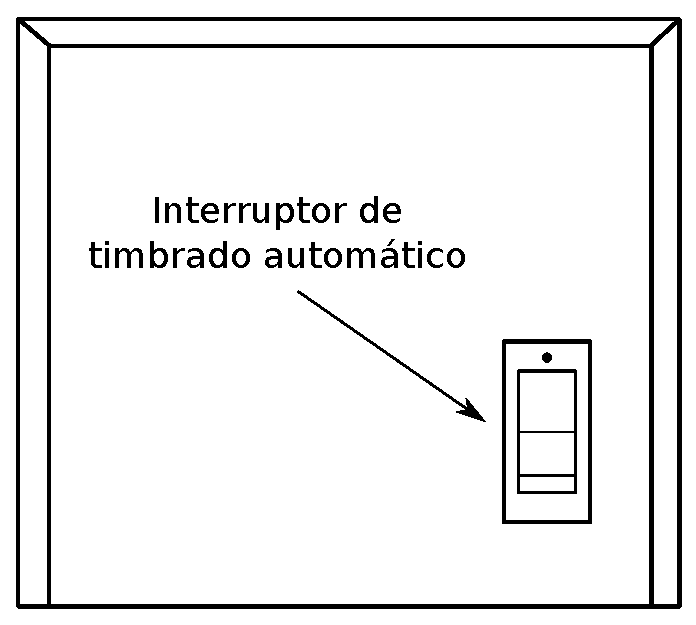
\includegraphics[width=0.6\textwidth]{./figuras/superior1.eps} 
        \end{center}
	\label{superior1}
\end{figure}


\newpage
\section{Pantalla principal}

En la pantalla principal se muestra la hora actual (Hora : Minutos : Segundos) en formato AM/PM  seguida del día de la semana. En la segunda linea se encuentra la hora y el día próximo timbrado.

\textit{Nota: Si no existe ninguna alarma programada en los tipos de horario o ningún tipo de horario está asignado a algún día de la semana, el espacio donde se encuentra la hora y el día del próximo timbrado aparecerá en blanco.}

\begin{figure}[ht] 
        \caption[Pantalla principal]{Pantalla principal}
        \begin{center}
                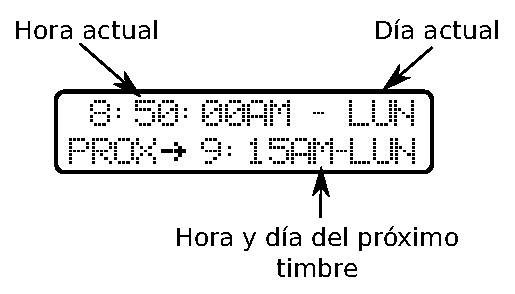
\includegraphics[width=8cm]{./figuras/lcd1.eps} 
        \end{center}
	\label{lcd1}
\end{figure}

\newpage
\section{Teclado de números y funciones}
Este teclado esta compuesto por una sección numérica y una sección de funciones. La tecla Enter (
\includegraphics[height=0.3cm]{./figuras/enter.eps}) se usa para aceptar alguna opción, para acceder a un menú o validar un cambio. Las teclas 
\includegraphics[height=0.3cm]{./figuras/fup.eps} y 
\includegraphics[height=0.3cm]{./figuras/fdown.eps} se usan como flechas arriba y abajo respectivamente para desplazarse entre el menú o diferentes opciones. Finalmente, la tecla 
\includegraphics[height=0.3cm]{./figuras/bmenu.eps} se usa para acceder o salir del Menú de configuración. 

Cada vez que se accede al menú la luz de fondo de la pantalla LCD se activa, al salir del menú, permanece activa esta luz por 10 segundos. La tecla asterisco (*) activa la luz por 10 segundos para poder visualizar los mensajes de la pantalla principal.

Por su parte la tecla \# activa el timbre cuando es presionada.

\begin{figure}[ht] % Se usa la [h] para que la imagen empiece forzada en el lugar donde inicia 

        \caption[Teclado de números y funciones]{Teclado de números y funciones}
        \begin{center}
                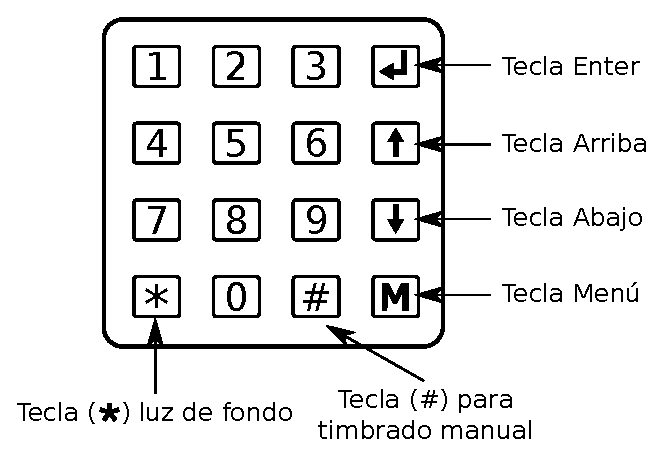
\includegraphics[width=8cm]{./figuras/teclado1.eps} % include ./img/imagen.[pdf|png|jgp] si es pdflatex o ./img/imagen.eps si es latex
        \end{center}
	\label{teclado1}
\end{figure}

\newpage
\section{Menú de configuración}

Con la tecla 
\includegraphics[height=0.3cm]{./figuras/bmenu.eps}, se accede al menú de configuración en el cual el usuario puede desplazarse por las diferentes opciones con la ayuda de las teclas 
\includegraphics[height=0.3cm]{./figuras/fup.eps} y 
\includegraphics[height=0.3cm]{./figuras/fdown.eps}, para acceder a la opción deseada se presiona la tecla 
\includegraphics[height=0.3cm]{./figuras/enter.eps}. El menú esta compuesto de las siguientes opciones que se describen en los capítulos posteriores.
\begin{itemize}
\item Fijar Reloj
\item Fijar Alarmas
\item Tipo de Horario
\item Contraseña
\item Dura. Timbres
\end{itemize}

\section{Interruptor de timbrado automático}

El interruptor de timbrado automático impide que el sistema cierre el contacto de potencia lo cual desactiva el timbrado automático programado, esta función ayuda a desactivar los timbres cuando el usuario lo desee por ejemplo en días feriados. El estado de encendido de este interruptor se distingue cuando este esta posicionado del lado del punto blanco.

\textit{Nota: Se recomienda colocar el Interruptor de timbrado automático en apagado al momento de conectar a la corriente eléctrica el Reloj MA 32-2 para evitar timbrados no deseados.}

\chapter{Fijar Reloj}

La opción Fijar Reloj permite ajustar la hora y la fecha actual, para ello se procede de la siguiente forma:
\begin{itemize}
\item Acceder al menú con el botón 
\includegraphics[height=0.3cm]{./figuras/bmenu.eps}.
\item Desplazarse hasta la opción Fijar Reloj con los botones 
\includegraphics[height=0.3cm]{./figuras/fup.eps} y 
\includegraphics[height=0.3cm]{./figuras/fdown.eps} y presionar el botón 
\includegraphics[height=0.3cm]{./figuras/enter.eps}.
\item Establecer la hora, los minutos y los segundos con la ayuda de el teclado numérico.
\item Fijar AM o PM con la ayuda de las teclas 
\includegraphics[height=0.3cm]{./figuras/fup.eps} y 
\includegraphics[height=0.3cm]{./figuras/fdown.eps} y luego presionar el botón 
\includegraphics[height=0.3cm]{./figuras/enter.eps}.
\item Fijar el día de la semana con las teclas 
\includegraphics[height=0.3cm]{./figuras/fup.eps} y 
\includegraphics[height=0.3cm]{./figuras/fdown.eps} y presionar finalmente el botón 
\includegraphics[height=0.3cm]{./figuras/enter.eps}.
\end{itemize}

Una vez presionado el botón 
\includegraphics[height=0.3cm]{./figuras/enter.eps} después de fijar el día de la semana la hora queda establecida. El Reloj MA 32-2 cuenta con una pila interna CR2032 la cual es capaz de almacenar la hora en caso de fallas de energía por hasta 10 años. Si al momento de el restablecimiento de la energía la hora no es la correcta es necesario cambiar esta pila.

\chapter{Fijar Alarmas}

La opción Fijar Alarmas permite ajustar los 30 timbrasos dentro de cada uno de los 4 tipos de horario. Primero se escoge el tipo de horario a modificar con la ayuda de las teclas 
\includegraphics[height=0.3cm]{./figuras/fup.eps} y 
\includegraphics[height=0.3cm]{./figuras/fdown.eps}, se lo selecciona con el botón 
\includegraphics[height=0.3cm]{./figuras/enter.eps}, luego la pantalla muestra la Figura \ref{lcdfalarmas} que indica el numero de la alarma, el tipo de horario a la que pertenece, la hora a la que está fijada ésta alarma, el tipo de timbrado y el estado de la alarma, apagada (OFF) o encendida (ON).

\begin{figure}[ht] 
        \caption[Pantalla fijar alarmas]{Pantalla fijar alarmas}
        \begin{center}
                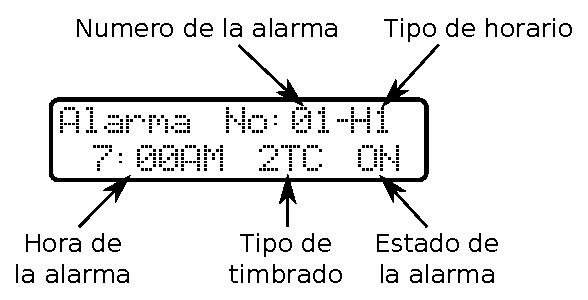
\includegraphics[width=8cm]{./figuras/lcdfalarmas.eps} 
        \end{center}
	\label{lcdfalarmas}
\end{figure}


Para desplazarse entre las alarmas se usan los botones 
\includegraphics[height=0.3cm]{./figuras/fup.eps} y 
\includegraphics[height=0.3cm]{./figuras/fdown.eps}, para fijar una alarma se pulsa el botón 
\includegraphics[height=0.3cm]{./figuras/enter.eps} estando en el numero de alarma que se desea modificar y se sigue este orden:
\begin{itemize}
\item Establecer la hora y los minutos de la alarma con la ayuda de el teclado numérico.
\item Fijar AM o PM con la ayuda de las teclas 
\includegraphics[height=0.3cm]{./figuras/fup.eps} y 
\includegraphics[height=0.3cm]{./figuras/fdown.eps} y luego presionar el botón 
\includegraphics[height=0.3cm]{./figuras/enter.eps}.
\item Fijar el tipo de timbrado con las teclas 
\includegraphics[height=0.3cm]{./figuras/fup.eps} y 
\includegraphics[height=0.3cm]{./figuras/fdown.eps} y luego presionar el botón 
\includegraphics[height=0.3cm]{./figuras/enter.eps}.
\item Fijar el estado de la alarma con las teclas 
\includegraphics[height=0.3cm]{./figuras/fup.eps} y 
\includegraphics[height=0.3cm]{./figuras/fdown.eps} en encendida (ON) o apagada (OFF) y finalmente presionar el botón 
\includegraphics[height=0.3cm]{./figuras/enter.eps}.
\end{itemize}

De esta misma forma se pueden fijar una o todas las alarmas. Cada vez que se configura una alarma estos datos quedan guardados en la memoria EEPROM del sistema lo que evita pérdida de los datos en caso de fallo de la energía.

\textit{Nota: No es necesario programar las alarmas en orden.	}

\section{Tipo de timbrado}

El Reloj MA 32-2 soporta 4 diferentes modos de timbrado, los cuales se describen a continuación:

\begin{itemize}
\item 1TC: 1 Timbre corto.
\item 1TL: 1 Timbre largo.
\item 2TC: 2 Timbres cortos.
\item 3TC: 3 Timbres cortos.
\end{itemize}

La duración de los intervalos de tiempo de los timbres se establecen con el menú Dura. Timbres, el cual se explica a continuación.

\newpage
\section{Dura. Timbres}

En el menú Dura. Timbres se establece la duración del timbre corto y del timbre largo, de la siguiente forma:

\begin{itemize}
\item Acceder al menú con el botón 
\includegraphics[height=0.3cm]{./figuras/bmenu.eps}.
\item Desplazarse hasta la opción Dura. Timbres con los botones 
\includegraphics[height=0.3cm]{./figuras/fup.eps} y 
\includegraphics[height=0.3cm]{./figuras/fdown.eps} y presionar el botón 
\includegraphics[height=0.3cm]{./figuras/enter.eps}.
\item Establecer con los botones 
\includegraphics[height=0.3cm]{./figuras/fup.eps} y 
\includegraphics[height=0.3cm]{./figuras/fdown.eps} la duración en segundos del timbre corto (TC) y presionar el botón 
\includegraphics[height=0.3cm]{./figuras/enter.eps}.
\item Establecer con los botones 
\includegraphics[height=0.3cm]{./figuras/fup.eps} y 
\includegraphics[height=0.3cm]{./figuras/fdown.eps} la duración en segundos del timbre largo (TL) y presionar finalmente el botón 
\includegraphics[height=0.3cm]{./figuras/enter.eps}.
\end{itemize}

\section{Tipo de horario}

El menú tipo de horario permite asignar el tipo de horario a cada día de la semana, asignando uno de los cuatro tipos de horario o ningún horario con la opción OFF a cada día. Para configurar se procede de la siguiente forma:

\begin{itemize}
\item Acceder al menú con el botón 
\includegraphics[height=0.3cm]{./figuras/bmenu.eps}.
\item Desplazarse hasta la opción Tipo de Horario con los botones 
\includegraphics[height=0.3cm]{./figuras/fup.eps} y 
\includegraphics[height=0.3cm]{./figuras/fdown.eps} y presionar el botón 
\includegraphics[height=0.3cm]{./figuras/enter.eps}.
\item Escoger el día que se desea modificar con los botones 
\includegraphics[height=0.3cm]{./figuras/fup.eps} y 
\includegraphics[height=0.3cm]{./figuras/fdown.eps} y presionar el botón 
\includegraphics[height=0.3cm]{./figuras/enter.eps}.
\item Seleccionar el tipo de horario con los botones 
\includegraphics[height=0.3cm]{./figuras/fup.eps} y 
\includegraphics[height=0.3cm]{./figuras/fdown.eps} y presionar el botón 
\includegraphics[height=0.3cm]{./figuras/enter.eps} para guardar.
\item Presionar el botón 
\includegraphics[height=0.3cm]{./figuras/bmenu.eps} para salir.
\end{itemize}


\chapter{Contraseña}

El Reloj MA 32-2 tiene la opción de proteger su configuración mediante una contraseña de 4 números. Para configurar una contraseña proceda de la siguiente forma:

\begin{itemize}
\item Acceda al menú con el botón 
\includegraphics[height=0.3cm]{./figuras/bmenu.eps}.
\item Desplazarse hasta la opción Contraseña con los botones 
\includegraphics[height=0.3cm]{./figuras/fup.eps} y 
\includegraphics[height=0.3cm]{./figuras/fdown.eps} y presionar el botón 
\includegraphics[height=0.3cm]{./figuras/enter.eps}.
\item Escoger si el sistema pide o no pide la contraseña con los botones 
\includegraphics[height=0.3cm]{./figuras/fup.eps} y 
\includegraphics[height=0.3cm]{./figuras/fdown.eps} y presionar el botón 
\includegraphics[height=0.3cm]{./figuras/enter.eps}.
\item Escribir los cuatro números de la contraseña.
\item Escribir nuevamente los cuatro números de la contraseña.
\end{itemize}

Una vez establecida la contraseña el Reloj MA 32-2 la pedirá cada vez que se acceda al menú, en donde existe un tiempo limite de 5 segundos para poderla escribir. Si se desea desactivar la contraseña se escoge NO a la pregunta pedir contraseña en este menú.

\textit{Nota: Si olvida la contraseña de seguridad debe desconectar el equipo y retirar la pila interna CR2032 durante al menos 10 segundos, esto borrara la contraseña y la hora actual.}


\chapter{Conexión de los timbres}

El Reloj MA 32-2 posee un conector de potencia el cual cierra el circuito cuando un timbrado es activado por una alarma o cuando se presiona la tecla \#. Este contacto soporta una corriente máxima de 15A en 100 a 240 VAC (1800W/3600W) y está esta protegido con un fusible de 15A.

Los timbres se deben conectar en paralelo con una rama al Neutro (N) de la instalación eléctrica y la otra rama al conector de potencia del Reloj MA 32-2, el otro contacto del conector de potencia debe ser conectado a la Linea (L) de la instalación eléctrica. Es muy importante que la instalación eléctrica soporte la corriente requerida por los timbres. El esquema de la Figura \ref{conpotencia} muestra de forma mas detallada la conexión.

\begin{figure}[ht] % Se usa la [h] para que la imagen empiece forzada en el lugar donde inicia \begin{figure}

        \caption[Esquema de conexión de timbres]{Esquema de conexión de timbres}
        \begin{center}
                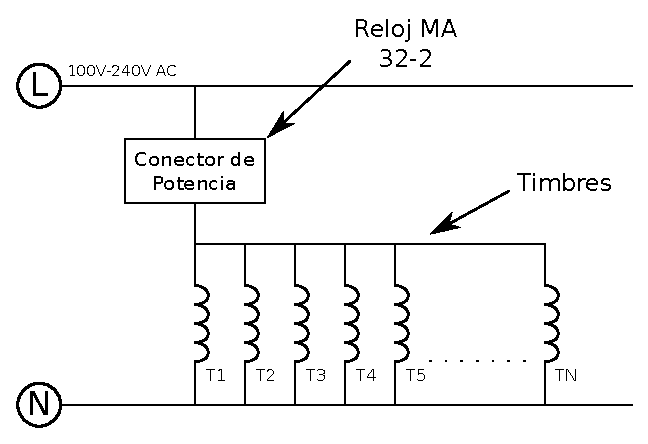
\includegraphics[width=8cm]{./figuras/conpotencia.eps} % include ./img/imagen.[pdf|png|jgp] si es pdflatex o ./img/imagen.eps si es latex
        \end{center}
	\label{conpotencia}
\end{figure}

Es muy importante calcular y medir la corriente que demanda la instalación de timbres que se tenga antes de conectar el Reloj MA 32-2, si la corriente demandada supera las características del Reloj MA 32-2 contacte a Galeras Digital para dar solución a sus nuevos requerimientos.

\textit{Nota: Galeras Digital no se hace responsable por daños causados debido a una instalación inadecuada o por fallas presentadas del fluido eléctrico.}

\chapter{Garantía}

Este producto esta garantizado por Galeras Digital al comprador original de estar libre de defectos en los materiales y fabricación bajo uso normal por un periodo de un año de la fecha de compra. Durante el periodo de garantía y con la factura de compra; el producto será reparado utilizando piezas de remplazo originales y si es el caso el producto será remplazado en su totalidad. Para obtener el servicio de garantía usted debe contactar a Galeras Digital y poseer una copia de su factura de compra que muestre la fecha de tal compra, usted no tendrá cargo por las piezas o la reparación.

El cliente NO tendrá reclamo alguno bajo esta garantía para gastos de reparaciones o ajustes si:

\begin{enumerate}
\item El problema es causado por un trato incorrecto, maltrato o descuido
\item Los sellos de garantía muestran señales de violación.
\item El problema es causado por un incendio u otro desastre natural.
\item El problema es causado por la reparación o ajuste inadecuado realizado por personas que no pertenecen a Galeras Digital.
\item El periodo de garantía ha expirado.
\end{enumerate}

\newpage

\section{Contactos}

Para contactar a Galeras Digital puede comunicarse al siguiente celular, correo electrónico o pagina web:
\
\\
\\
\begin{itemize}
\item\textbf{Ventas y soporte técnico:}
\subitem\textbf{- Juan Pablo Ruiz:} 301 323 4324
\subitem \hspace{0.5cm}(Cajicá - Colombia)
\item\textbf{Correo electrónico:} galerasdigital@gmail.com
\item\textbf{Pagina web:}\\ \url{http://www.galerasdigital.com}
\end{itemize}

\vspace{1cm}
\begin{tiny}\textit{M/V: 3.03-30x4/01/10/14}\end{tiny}\\
\begin{tiny}\textit{F/V: 30x4-06/12}\end{tiny}

\newpage
\pagestyle{empty}
\ \\
\vspace{3cm}
\begin{center}
 
\includegraphics[width=9.41cm]{figuras/tapaf.eps}
 % tapaf.eps: 1111x654 pixel, 300dpi, 9.41x5.54 cm, bb=0 0 267 157
\end{center}




\end{document}

